% !TeX spellcheck = en_US
\chapter{Generative Models}

\section{Definitions}
\label{sec:vae-defs}
\begin{itemize}
	\item \textit{Probabilistic model}: is a model that represents a probability distribution. It could be a marginal \ac{prob} distribution $p(x)$ or a conditional \ac{prob} distribution $p(y|x)$.
	\item \textit{Evidence, query, and latent variables}:\\
	The word \hlb{latent} implies \hlb{existing, but hidden}. \Eg:
	\begin{itemize}
		\item In $p(x)$, $x$ is the query variable and there is no evidence variable.
		\item In $p(y|x)$, $y$ is the query variable and $x$ is the evidence variable.
		\item In \ac{MoG} $p(x) = \sum_z p(x|z) p(z)$, $x$ is the query variable, $z$ is the latent variable to represent the mixture elements.		
		\item In $p(y|x) = \sum_z p(y|x,z) p(z)$, $z$ is the latent variable.
		\item In a neural network, the inputs are evidence variables, the output are the query variables. In \ac{VAE}, $z$ is considered as the latent variable with a simple Gaussian distribution.
		\item In model-based \ac{RL} with latent variable models, state $x_t$ is the latent variable.
	\end{itemize}
	\item \textit{Latent variable models}: is the type of probabilistic model that represent a complex \ac{pdf} as the product of multiple simpler \ac{pdf}s, one of which belongs to a latent variable.\\
	\Eg: in \ac{VAE}, the complex distribution $p(x)$ (of an image) is represented as the product of two simple distribution. $p(z)$ is a Gaussian distribution, and $p(x|z)$ as a learnable neural network
	\[ p(x) = \int p(x|z) p(z) dz \]
\end{itemize}

\section{Variational Inference}
\hlb{Goal:} to model a complex distribution $p_\theta(x)$, given the data $\mathcal{D} = \{ x_1, \dots, x_N \}$
\begin{align}
	&\text{Maximum likelihood fit:} && \theta \leftarrow \underset{\theta}{\arg\max} \frac{1}{N} \sum_i \log p_\theta(x_i)\\
	&\text{With latent variable $z$:} && p(x) = \int p(x|z) p(z) dz\\
	\Rightarrow &\text{(sadly, completely \hlb{intractable})} && \theta \leftarrow \underset{\theta}{\arg\max} \frac{1}{N} \sum_i \log \left( \int p(x|z) p(z) dz \right)\\
	\Rightarrow &\text{alternative: \textit{expected} log-likelihood} && \theta \leftarrow \underset{\theta}{\arg\max} \frac{1}{N} \mathbb{E}_{z\sim p(z|x_i)} [\log p_\theta (x_i, z)]
\end{align}
This section describes how to calculate $p(z|x_i)$

\subsection{The Variational Approximation}
\hlb{Idea:} Approximating $p(z|x_i)$ with $q_i(z) = \mathcal{N}(\mu_i, \sigma_i)$

\begin{align}
	\log p(x_i) &= \log \int_z p(x_i|z) p(z) dz\\
	&= \log \int_z p(x_i|z) p(z) \frac{q_i(z)}{q_i(z)} dz\\
	&= \log \mathbb{E}_{z\sim q_i(z)} \left[ \frac{p(x_i|z) p(z)}{q_i(z)} \right]\\
	&\geq \mathbb{E}_{z\sim q_i(z)} \left[ \log \frac{p(x_i|z) p(z)}{q_i(z)} \right] \qquad(\text{Jensen's inequality: $\log \mathbb{E}[y] \geq \mathbb{E}[\log y]$})\\
	&= \mathbb{E}_{z\sim q_i(z)} [\log p(x_i|z) + \log p(z)] - \mathbb{E}_{z\sim q_i(z)}[\log q_i(z)]\\
	&= \underbrace{\mathbb{E}_{z\sim q_i(z)} [\log p(x_i|z) + \log p(z)] + \mathcal{H}(q_i)}_{\textstyle \mathcal{L}_i (p, q_i)}
\end{align}

\begin{itemize}
	\item $\mathbb{E}_{z\sim q_i(z)} [\log p(x_i|z) + \log p(z)] + \mathcal{H}(q_i)$ is the lower bound of $\log p(x_i)$.\\
	Thus, maximize $\mathbb{E}_{z\sim q_i(z)} [\log p(x_i|z) + \log p(z)] + \mathcal{H}(q_i)$ will indirectly maximize $\log p(x_i)$.
	\item Maximize the 1st term $\mathbb{E}_{z\sim q_i(z)} [\log p(x_i|z) + \log p(z)]$ will find the place with high $p(x_i, z)$\\
	Maximize the 2nd term $\mathcal{H}(q_i)$ will increase the randomness of $z$
\end{itemize}

In another point of view, as we approximate $p(z|x_i)$ with $q_i(z)$, the \ac{KL}-divergence $D_{KL}(q_i(z) || p(z|x_i))$ can measure how good is the approximation:

\begin{align}
	D_{KL}(q_i(z) || p(z|x_i)) &= \mathbb{E}_{z\sim q_i(z)} \left[ \log\frac{q_i(z)}{p(z|x_i)} \right] = \mathbb{E}_{z\sim q_i(z)} \left[ \log\frac{q_i(z)p(x_i)}{p(x_i, z)} \right]\\
	&= - \mathbb{E}_{z\sim q_i(z)} [ \log p(x_i|z) + \log p(z) ] + \mathbb{E}_{z\sim q_i(z)} [\log q_i(z)] + \mathbb{E}_{z\sim q_i(z)} [\log p(x_i)]\\
	&= - \underbrace{\mathbb{E}_{z\sim q_i(z)} [ \log p(x_i|z) + \log p(z) ] - \mathcal{H}(q_i)}_{\textstyle \mathcal{L}_i (p, q_i)} + \log p(x_i)\\
	\Rightarrow\; \log p(x_i) & = D_{KL}(q_i(z) || p(z|x_i)) + \mathcal{L}_i (p, q_i)\\
	\Rightarrow\; \log p(x_i) & \geq \mathcal{L}_i (p, q_i), \qquad \text{since } D_{KL}(q||p) \geq 0
\end{align}

In addition, since $\log p(x_i)$ is independent of $q_i$, maximizing $\mathcal{L}_i (p, q_i)$ \ac{wrt} $q_i$ will minimize the \ac{KL}-divergence.

\subsection{Algorithm}
Again, the goal is to model the complex distribution $p(x)$. Since the common maximum likelihood is intractable, we maximize its lower bound.
\begin{align*}
	& \theta \leftarrow \underset{\theta}{\arg\max} \frac{1}{N} \sum_i \log p_\theta(x_i) &&- \text{intractable maximum likelihood}\\
	& \theta \leftarrow \underset{\theta}{\arg\max} \frac{1}{N} \sum_i \mathcal{L}_i(p, q_i) &&- \text{tractable lower bound}
\end{align*}

\hlb{The algorithm:}
\begin{enumerate}
	\item for each $x_i$ (or mini-batch):
	\item \quad calculate $\nabla_\theta \mathcal{L}_i (p, q_i)$:
	\item \qquad sample $z \sim q_i(z)$
	\item \qquad $\nabla_\theta \mathcal{L}_i (p, q_i) \approx \nabla_\theta \log p_\theta (x_i | z)$
	\item \quad $\theta \leftarrow \theta + \alpha \nabla_\theta \mathcal{L}_i (p, q_i)$
	\item \quad update $q_i$ to maximize $\mathcal{L}_i (p, q_i)$
\end{enumerate}

In the above $6^{th}$ step, assuming $q_i(z) = \mathcal{N}(\mu_i, \sigma_i)$:
\begin{itemize}
	\item calculate the gradient $\nabla_{\mu_i} \mathcal{L}_i (p, q_i)$ and $\nabla_{\sigma_i} \mathcal{L}_i (p, q_i)$
	\item apply gradient ascent on $\mu_i$ and $\sigma_i$ to maximize $\mathcal{L}_i (p, q_i)$.
\end{itemize}

\hlb{Problem:} for each $x_i$, there will be one $\mu_i$ and one $\sigma_i$, with the appropriate dimension. Thus, the total number of \ac{param} would be huge: $|\theta| + (|\mu_i| + |\sigma_i|) \times N$

\section{Amortized Variational Inference}
The word \textit{amortize} means to reduce or pay off (a debt) with regular payments.

As mentioned above, the problem with using a Gaussian for $q_i(z)$ is the huge number of \ac{param}. This section proposes an alternative, which is to use a neural network (\figref{fig:amortized-variational-inference})
\begin{align}
	&q_i(z) = q(z | x_i) \approx q_\phi(z|x) = \mathcal{N}(\mu_\phi(x), \sigma_\phi(x))\\
	\Rightarrow\;& \log p(x_i) \geq \underbrace{\mathbb{E}_{z\sim q_\phi(z|x_i)} [ \log p_\theta(x_i|z) + \log p(z) ] + \mathcal{H}(q_\phi(z|x_i))}_{\textstyle \mathcal{L}_i (p_\theta(x_i|z), q_\phi(z|x_i))}
\end{align}

\begin{figure}[hbt!]
	\centering
	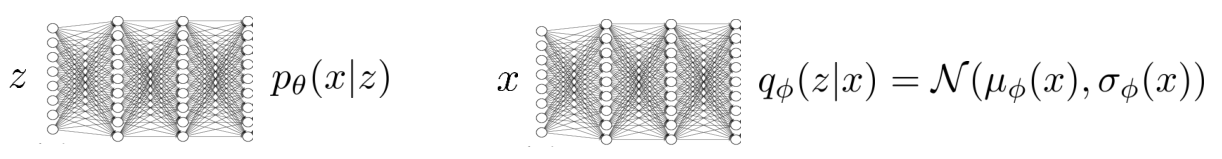
\includegraphics[width=\textwidth]{amortized-variational-inference.png}
	\caption{Two neural networks: $p_\theta(x|z)$ and $q_\phi(z|x)$.}
	\label{fig:amortized-variational-inference}
\end{figure}

\subsection{Algorithm}
\hlb{The algorithm:}
\begin{enumerate}
	\item for each $x_i$ (or mini-batch):
	\item \quad calculate $\nabla_\theta \mathcal{L}_i (p_\theta(x_i|z), q_\phi(z|x_i))$:
	\item \qquad sample $z \sim q_\phi(z|x_i)$
	\item \qquad $\nabla_\theta \mathcal{L} \approx \nabla_\theta \log p_\theta(x_i|z)$
	\item \quad $\theta \leftarrow \theta + \alpha \nabla_\theta \mathcal{L}$
	\item \quad $\phi \leftarrow \phi + \alpha \nabla_\phi \mathcal{L}$
\end{enumerate}

Let's consider the gradient $\nabla_\phi \mathcal{L}$ in the above $6^{th}$ step:
\begin{align}
	\mathcal{L}_i &= \underbrace{\mathbb{E}_{z\sim q_\phi(z|x_i)} \big[\log p_\theta(x_i|z) + \log p(z)\big]}_{\textstyle J(\phi) = \mathbb{E}_{z\sim q_\phi(z|x_i)} \big[ r(x_i, z)\big]} + \mathcal{H}(q_\phi(z|x_i))\\
	&= \nabla_\phi J(\phi) + \nabla_\phi \mathcal{H}(q_\phi(z|x_i))
\end{align}

\begin{itemize}
	\item There is a formula to find the gradient of the entropy of a Gaussian
	\begin{equation}
		\nabla_\phi \mathcal{H}(q_\phi(z|x_i)) = \nabla_\phi \mathcal{H} \big(\mathcal{N}(\mu_\phi, \sigma_\phi)\big)
	\end{equation}	
	\item To find the gradient $\nabla_\phi J(\phi)$, we could use similar approach as in policy gradient, however, with the problem of high variance. Instead, we could use the reparameterization trick:
	\begin{align}
		J(\phi) & = \mathbb{E}_{z\sim q_\phi(z|x_i)} \big[ r(x_i, z)\big] && q_\phi(z|x) = \mathcal{N}(\mu_\phi(x), \sigma_\phi(x))\\
		& = \mathbb{E}_{\epsilon \sim \mathcal{N}(0,1)} \big[ r(x_i, \mu_\phi(x) + \epsilon \sigma_\phi(x))\big] && z = \mu_\phi(x) + \epsilon \sigma_\phi(x)
	\end{align}
	with $\epsilon \sim \mathcal{N}(0,1)$ is independent of $\phi$!\\
	$\Rightarrow$ estimate $\nabla_\phi J(\phi)$:
	\begin{itemize}
		\item sample $\epsilon_1, \dots, \epsilon_M$ from $\mathcal{N}(0,1)$ (a single sample works just well!)
		\item $\nabla_\phi J(\phi) \approx \frac{1}{M} \sum_j \nabla_\phi r(x_i, \mu_\phi(x) + \epsilon \sigma_\phi(x))$
	\end{itemize}
\end{itemize}

\begin{figure}[hbt!]
	\centering
	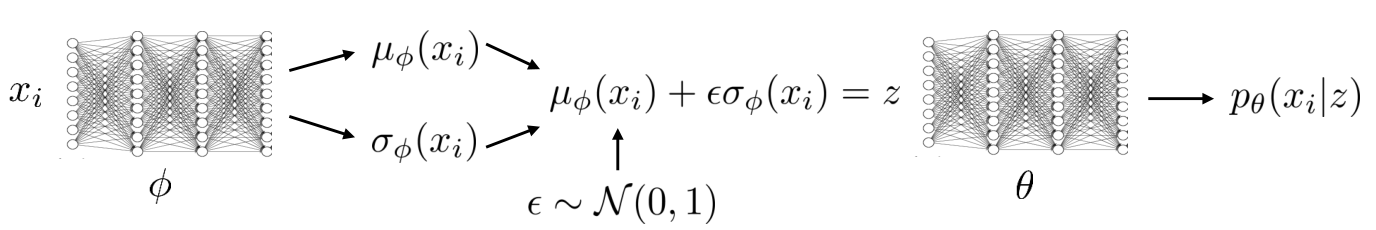
\includegraphics[width=\textwidth]{VAE.png}
	\caption{The complete structure for amortized variational inference.}
	\label{fig:vae}
\end{figure}

\subsection{Reparameterization Trick}
Another way to look:
\begin{align}
	\mathcal{L}_i &= \mathbb{E}_{z\sim q_\phi(z|x_i)} \big[\log p_\theta(x_i|z) + \log p(z)\big] + \mathcal{H}(q_\phi(z|x_i))\\
	&= \mathbb{E}_{z\sim q_\phi(z|x_i)} [\log p_\theta(x_i|z)] + \mathbb{E}_{z\sim q_\phi(z|x_i)}[\log p(z)] + \mathcal{H}(q_\phi(z|x_i))\\
	&= \mathbb{E}_{z\sim q_\phi(z|x_i)} [\log p_\theta(x_i|z)] -D_{KL} (q_\phi(z|x_i) || p(z))\\
	&= \mathbb{E}_{\epsilon \sim \mathcal{N}(0,1)} \big[\log p_\theta(x_i|\mu_\phi(x) + \epsilon \sigma_\phi(x))\big] -D_{KL} (q_\phi(z|x_i) || p(z))\\
	&\approx \log p_\theta(x_i|\mu_\phi(x) + \epsilon \sigma_\phi(x)) -D_{KL} (q_\phi(z|x_i) || p(z)) \quad \text{(single sample estimate)}
\end{align}

\note Reparameterization trick \ac{vs} policy gradient
\begin{itemize}
	\item Policy Gradient
	\[\nabla_\phi J(\phi) \approx \frac{1}{M} \sum_j \nabla_\phi \log q_\phi(z_j|x_i) r(x_i, z_j) \]
	$\begin{matrix*}[l]
		\color{Green} + \text{can handle both discrete and continuous latent variables}\\
		\color{red} - \text{high variance, requires multiple samples \& small learning rates}
	\end{matrix*}$
	\item Reparameterization trick
	\[\nabla_\phi J(\phi) \approx \frac{1}{M} \sum_j \nabla_\phi r(x_i, \mu_\phi(x) + \epsilon \sigma_\phi(x))\]
	$\begin{matrix*}[l]
		\color{red} - \text{only continuous latent variables}\\
		\color{Green} + \text{very simple to implement}\\
		\color{Green} + \text{low variance}
	\end{matrix*}$
\end{itemize}

\section{Conditional Variational Inference Models}
\begin{equation}
	\mathcal{L}_i = \mathbb{E}_{z\sim q_\phi(z|x_i, y_i)} \big[\log p_\theta(y_i|x_i, z) + \log p(z|x_i)\big] + \mathcal{H}(q_\phi(z|x_i, y_i))\\
\end{equation}
\begin{figure}[hbt!]
	\centering
	\includegraphics[width=\textwidth]{conditional-VAE.png}
	\caption{The conditional model.}
	\label{fig:conditional-vae}
\end{figure}

\section{Generative Models}
\textit{Generative models} are models that generate data $x$. \Eg: $p(x)$ is a generative model, because knowing $p(x)$, we can sample $x$.

\note Not all generative models are not necessary latent variable models, and not all latent variable models are generative models. But it's common for a generative model to be a latent variable model, because sometimes, to generate data, we usually want to know the \ac{prob} distribution of it. When that \ac{prob} distribution is complex, we would represent it as a product of multiple simple \ac{prob} distribution, using some latent variables.

\subsection{Generative Adversarial Network}
\todo{\ac{GAN}}

\section{References}
\begin{itemize}
	\item \href{https://youtu.be/UTMpM4orS30}{Variational Inference | CS 285, Stanford | YouTube}
	\item \href{https://youtu.be/5WoItGTWV54}{Generative models | CS231, Stanford | YouTube}
	\item \href{https://youtu.be/9zKuYvjFFS8}{Variational Autoencoders | Arxiv Insights | YouTube}
	\item \href{https://youtu.be/fcvYpzHmhvA}{Variational Autoencoders | CodeEmporium | YouTube}
	\item \href{https://github.com/vdumoulin/conv_arithmetic}{Real "deconv" layer | GitHub}
\end{itemize}